\documentclass[rutwik_proposal.tex]{subfiles}

\begin{document}

\chapter{Literature Review}\label{ch:litrev}

Over the past two years, my ideas have evolved rapidly in response to the literature I have come across and because of the conversations I have had with experts in disparate fields. In this chapter, I will present and discuss some of the literature that has influenced me most.

My thoughts have been shaped immensely by reading about different approaches to conservation that have been undertaken and by what I consider to be their drawbacks. These perceived drawbacks might at times have something to do with the underlying philosophies or with the methods used, but the biggest shortcoming is that they have largely been unable to achieve their desired outcomes on a large scale. I believe that this is because these approaches do not take societies and social forces into consideration even though the issues that conservationists have to deal with seem to be a direct result of the behavior of societies. In order to address this, we need to understand how societies work; why they behave how they behave and why individuals in societies make the decisions that they do.

This chapter will provide a brief introduction to some of the major schools of thought in conservation, the methods they have used, and the shortcomings of these methods. It will also introduce social norms, which are probably the most significant of the social forces that drive the behavior of individuals within societies; and thus, of societies themselves. Through this chapter, I hope to motivate the questions that I am going to begin addressing during my time here at Princeton.

\section{A Brief History of Conservation}\label{sec:history}

The history of conservation in the US is long, complicated, and involves a number of different actors advocating for different ideals, goals, and approaches. However, for a fairly straightforward and deceptively linear timeline, see figure \ref{fig:cons_timeline}. I will follow this timeline in this section merely to simplify matters. Nonetheless, it is important to note that the picture is not as simple and clear cut as the figure makes it out to be. For example, as early as the late nineteenth and early twentieth centuries, Gifford Pinchot, Theodore Roosevelt, and many others were already advocating strongly for the 'nature for people' approach to conservation \cite{Pinchot98, Pinchot10, Brinkley09}. The recent debate between proponents of 'nature for itself' against those who propose more utilitarian and economic standards was already playing out between seminal figures like Pinchot and John Muir \cite{Righter05}.

\begin{figure}[h]
\centering
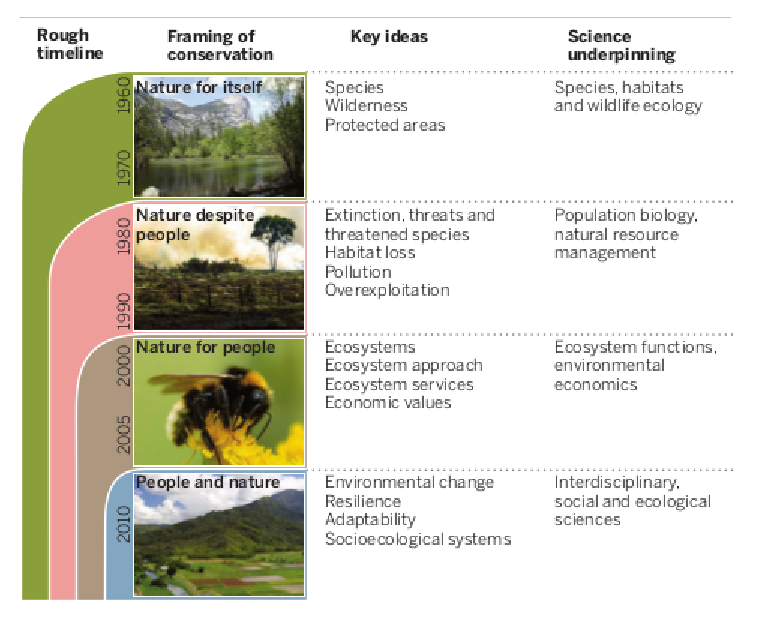
\includegraphics{Images/constimeline}
\caption{A very simplified timeline of conservation in the US\cite{Mace14}}
\label{fig:cons_timeline}
\end{figure}

\subsection{Nature for itself}\label{subsec:intrinsicvals}
The basis for a lot of the efforts before the 1970s was the misguided 'Nature for itself' philosophy. According to this philosophy, 'wilderness' is nature untouched by the hands of men. The intrinsic value of life is a central tenet of this line of thought. The 'nature for itself' ideology was promoted by early preservationists such as John Muir and Henry David Thoreau \cite{Muir1901, Thoreau06}. Approaches emerging out of this way of thinking included the designation of national parks and the protection of endangered species. These approaches are still evident today, especially in areas of the world that are most vulnerable to large losses in biodiversity and forest cover. In fact, E.O. Wilson, in his most recent book \textit{Half-Earth: Our Planet's Fight for Life}, suggests that in order to stave off the cataclysmic mass extinction event facing us today, we need to set aside about half of our planet's surface as a permanent nature preserve \cite{Wilson16}.

Notwithstanding the legal, political, and logistical difficulties involved in designing and creating nature preserves on which different levels of human use are permissible, there is ample evidence to prove that this underlying view of wilderness as untramelled nature itself is grossly incorrect. In the United States, Native Americans had been managing and molding land for their uses for centuries \cite{Langston95, Steinberg13, Butzer99}. Management techniques mostly included the use of fire. Besides playing an important role in agriculture, these fires served predominantly two additional purposes: ensuring fresh grass for their large herds of horses to graze on, and to promote the growth of herbs, berries, and other forage which would lure game animals in \cite{Langston95, Pyne82}. A number of the grasslands, prairies, and open pine forests that early explorers were so attracted to and felt so strongly inclined to preserve can, to some extent, be attributed to the Indian fires.

In addition to painting a false picture of nature and humans' place in it, the nature for itself approach in many cases ends up adversely affecting the people who most heavily depend on it for their livelihoods. A number of journalists, environmental policy scholars, and environmental historians have criticized conservation efforts for displacing populations of native people and people who are forced into homesteading because of socio-economic reasons \cite{Agrawal09, Dowie06, Johnson99}. This often leads to feelings of resentment against conservation organizations and government bodies amongst the local people. Sometimes, the extreme discontent engendered amongst locals causes them to take strong retaliatory anti-conservation actions such as burning down large swathes of designated national parks (personal communication with Benjamin H. Johnson, an environmental historian). The recent standoff in Malheur is also evidence of disenchanted ranchers and other affected people reacting to exclusionary federal government policies \cite{Langston16}. The checkered history of national parks throughout the world often includes severe human rights violations that are very rarely brought up when discussing the history of conservation.

Due to the negative effects it has on local people's attitudes towards conservation and because the underlying ideology only serves to further the incorrect notion of human societies and nature being wholly seperate entities, the methods resulting from the nature for itself line of thought cannot provide sustainable conservation options. Unless we understand that all of life on earth is closely linked and that we are all simply components of a large, complex adaptive system, there will be little realization of the need for conservation. There will be limited public support for conservation, particularly when our methods are turning large sections of society against conservation. While arguments concerning the intrinsic value of life are important and useful, they alone cannot suffice. Despite this having been the most prevalent conservation philosophy for well over the past hundred years, we are still facing a mass extinction event of an unprecedented scale \cite{Stuart04, Barnosky11, Dirzo14}. That is not to say that national parks and nature preserves have not been at all successful or that we should completely abandon them. There is plenty of evidence to show that without them, we would probably be facing even greater biodiversity losses \cite{Rodrigues06, Hoffman11, Hoffman10, Chape05}. However, by the end of the 1960s and in the early 70s, conservationists had begun to realize that it was imperative that they came up with better, more inclusive ways of doing conservation. They realized that threre needed to be a greater recognition of how our natural systems affect us and how we affect them.

This led to the next prominent phase in the history of conservation. Beginning in the late 1970s, there was a shift in thinking from the 'nature for itself' or 'nature without people' approach to a 'nature despite people' approach. This marked the recognition and consideration of the often deleterious effects that human activities have on nature.

\end{document}